% kuleuventheme2 by Janez Kren, September 2017, janez.kren@kuleuven.be, based on:
% kuleuventheme 1.3 by Roland Pastorino, 2013 roland.pastorino@kuleuven.be / www.rolandpastorino.com

\PassOptionsToPackage{usenames, table, dvipsnames}{xcolor} % 
\documentclass[11pt,t]{beamer}
\usetheme{kuleuven2}	%THEME OPTIONS for LOGO: kul (default), kulak, lrd,    ; OPTIONS for TITLE PAGE: normal (default), sedes


%%% OTHER SETTINGS
\usefonttheme[onlymath]{serif}			% math font with serifs, delete to make it sans-serif
\setbeamertemplate{footline}[body] 		% delete this line to remove footline bar on all frames
%\usepackage[orientation=landscape,size=custom,width=16,height=9,scale=0.5,debug]{beamerposter} %enable for widescreen 16:9 ratio
%\titlegraphic{ \includegraphics[width=.2\paperwidth]{mytitlepagepic.png} } %optional title page image


\usepackage[english]{babel}
\usepackage{amsfonts}
\usepackage{amssymb}

\usepackage{pythonhighlight}

\usepackage[orientation=landscape,size=custom, width=16,height=9,scale=0.5,debug]{beamerposter} 

\definecolor{mygray}{rgb}{0.8,0.8,0.8}
\newcommand{\inline}[1]{ \colorbox{mygray}{\lstinline{#1}}}

\usepackage{xcolor}

\usepackage{layouts} % To get text/page width

\usepackage{listings}
\definecolor{codegreen}{rgb}{0,0.6,0}
\definecolor{codegray}{rgb}{0.5,0.5,0.5}
\definecolor{codepurple}{rgb}{0.58,0,0.82}
% \definecolor{backcolour}{rgb}{0.95,0.95,0.92}
\definecolor{backcolour}{rgb}{0.93,0.93,0.95}
\lstdefinestyle{mystyle}{
    backgroundcolor=\color{backcolour},   
    commentstyle=\color{codegreen},
    keywordstyle=\color{magenta},
    numberstyle=\tiny\color{codegray},
    stringstyle=\color{codepurple},
    basicstyle=\ttfamily\footnotesize,
    breakatwhitespace=false,         
    breaklines=true,                 
    captionpos=b,                    
    keepspaces=true,                 
    numbers=left,                    
    numbersep=5pt,                  
    showspaces=false,                
    showstringspaces=false,
    showtabs=false,                  
    tabsize=2
}
\lstset{style=mystyle}

%%% ADDED BY ALEX (stop)


%%% TITLE PAGE INFO:
\title[Geavanceerde Computerarchitectuur 1$^{\text{st}}$ session]{Geavanceerde Computerarchitectuur 1$^{\text{st}}$ session} %[]] will appear in footline
\subtitle{GPGPU programming, course info, exercise description}

\author{Joris Putteneers, {\footnotesize joris.putteneers@kueluven.be}}
\institute{DRAMCO}
\date{Academic year 2026/27}




\begin{document}
\csname beamer@calculateheadfoot\endcsname %recalculate head and foot dimension


 %%
 %%  0. TITLE PAGE and TABLE OF CONTENT
 %%
% Title page
\begin{frame}[plain,noframenumbering]
	\titlepage
\end{frame}
	

% Table of Contents
\begin{frame}{Outline}
	\hfill	{\large \parbox{.961\textwidth}{\tableofcontents[hideothersubsections]}}
\end{frame}







%%
%%  SECTION 1 - INFO
%%
\section{Course intro and info}



\begin{frame}{GPUs can execute more threads simultaneously} 
    \begin{figure}[t]
        \centering
        \begin{center}               
            \resizebox{0.98\columnwidth}{!}{

\begin{tikzpicture}[]


%%% DEFINITIONS %%%%%%%%%%%%%%%%%%%%%%%%%%%%%%%%%%%%%%%%%%%%%%%%%%%%%%%%%%%%%


% https://associatie.kuleuven.be/huisstijl/kleuren
\definecolor{blue1}{RGB}{82,189,236}
\definecolor{blue2}{RGB}{0,64,122}
\definecolor{blue3}{RGB}{31,171,231}
\definecolor{blue4}{RGB}{29,141,176}
\definecolor{blue5}{RGB}{17,110,138}
\definecolor{orange1}{RGB}{221,138,46}


\def\ThPoolCenterOneX{-2}
\def\ThPoolCenterOneY{0}

\def\ThPoolCenterTwoX{2}
\def\ThPoolCenterTwoY{0}


%%% DRAWING %%%%%%%%%%%%%%%%%%%%%%%%%%%%%%%%%%%%%%%%%%%%%%%%%%%%%%%%%%%%%%%%%

\node at (0, 3) {\LARGE Process};

\draw [black] (0,0) ellipse (8 and 4);


\node [align=center] at (-10, 2) {\large CPU \\ \large thread pool};
\node [align=center] at (+10, 2) {\large GPU \\ \large thread pool};

\draw (-8.25,1.7) -- (-6,1);
\draw (8.25,1.7) -- (6,1);

\filldraw [blue1, opacity=0.1] (\ThPoolCenterOneX-2,\ThPoolCenterOneY) circle (2.8);
\filldraw [blue2, opacity=0.1] (\ThPoolCenterTwoX+1.8,\ThPoolCenterOneY) circle (2.8);
\draw [blue1] (\ThPoolCenterOneX-2,\ThPoolCenterOneY) circle (2.8);
\draw [blue2] (\ThPoolCenterTwoX+1.8,\ThPoolCenterOneY) circle (2.8);


\foreach \x in {1,...,3} {
    \node[inner sep=0pt] at (\ThPoolCenterOneX-\x, 1.5){
\includegraphics[width=1em]{figure/session-1/thread-small.png}};
}
\foreach \x in {0,...,4} {
    \node[inner sep=0pt] at (\ThPoolCenterOneX-\x, 0){
\includegraphics[width=1em]{figure/session-1/thread-small.png}};
}
\foreach \x in {1,...,3} {
    \node[inner sep=0pt] at (\ThPoolCenterOneX-\x, -1.5){
\includegraphics[width=1em]{figure/session-1/thread-small.png}};
}


\foreach \x in {1,...,6} {
    \node[inner sep=0pt] at (\ThPoolCenterTwoX+\x/2, 1.5){
\includegraphics[width=1em]{figure/session-1/thread-small.png}};
}
\foreach \x in {-1,...,8} {
    \node[inner sep=0pt] at (\ThPoolCenterTwoX+\x/2, 0){
\includegraphics[width=1em]{figure/session-1/thread-small.png}};
}
\foreach \x in {1,...,6} {
    \node[inner sep=0pt] at (\ThPoolCenterTwoX+\x/2, -1.5){
\includegraphics[width=1em]{figure/session-1/thread-small.png}};
}


\draw [->] (-8.5,0) to [out=180,in=90] (-10,-2.5);
\draw [->] (+8.5,0) to [out=0,in=90] (+10,-2.5);

\node [align=center] at (-11.5, -0.5) {Map threads \\ to CPU cores};
\node [align=center] at (+11.5, -0.5) {Map threads \\ to GPU cores};

\node[inner sep=0pt] at (-10, -5){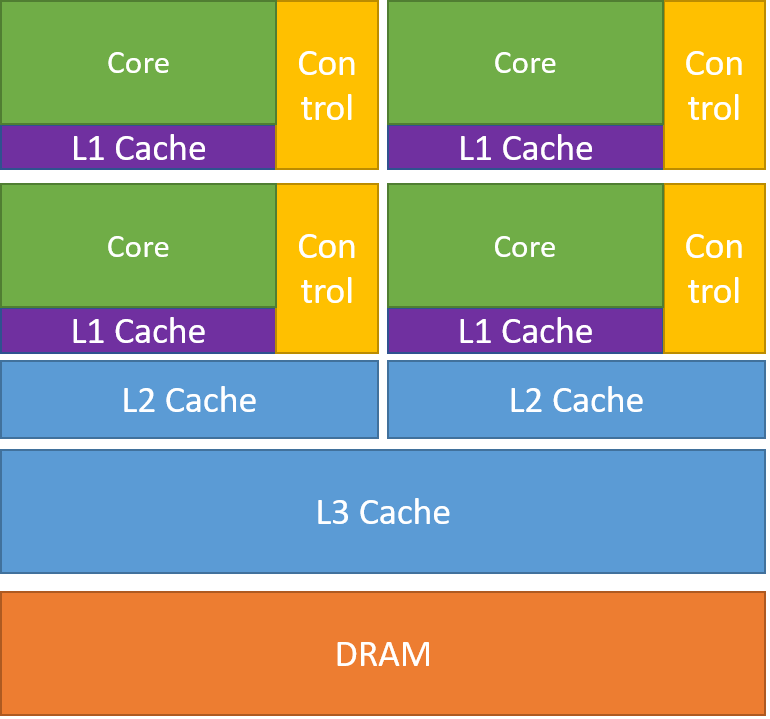
\includegraphics[width=10em]{figure/session-1/cpu-architecture.png}};

\node[inner sep=0pt] at (+10, -5){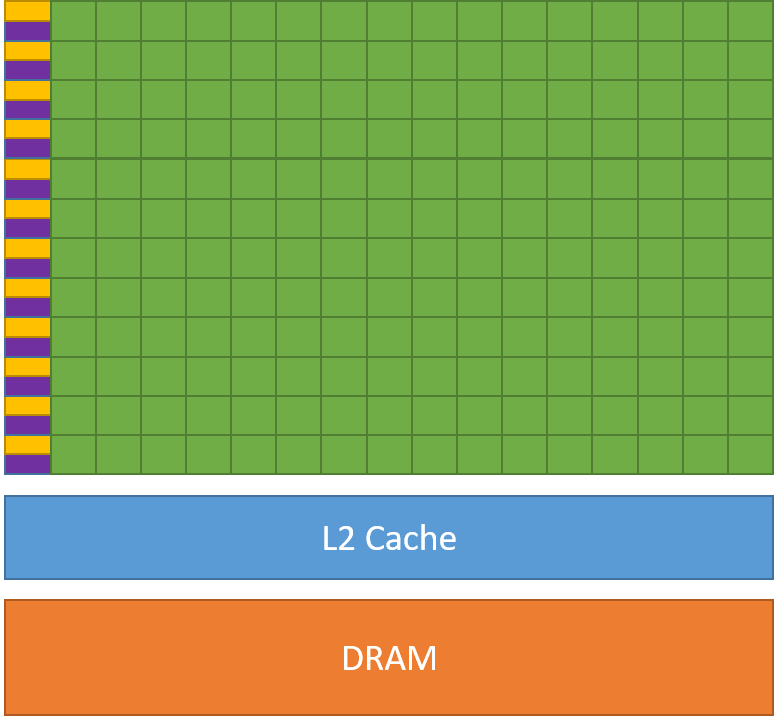
\includegraphics[width=10em]{figure/session-1/gpu-architecture.png}};



\end{tikzpicture}}
        \end{center}
    \end{figure}
\end{frame}



\begin{frame}{Example: parallel processing for ray tracing} 
    \vspace{-.5 em}
    \begin{figure}
        \centering
        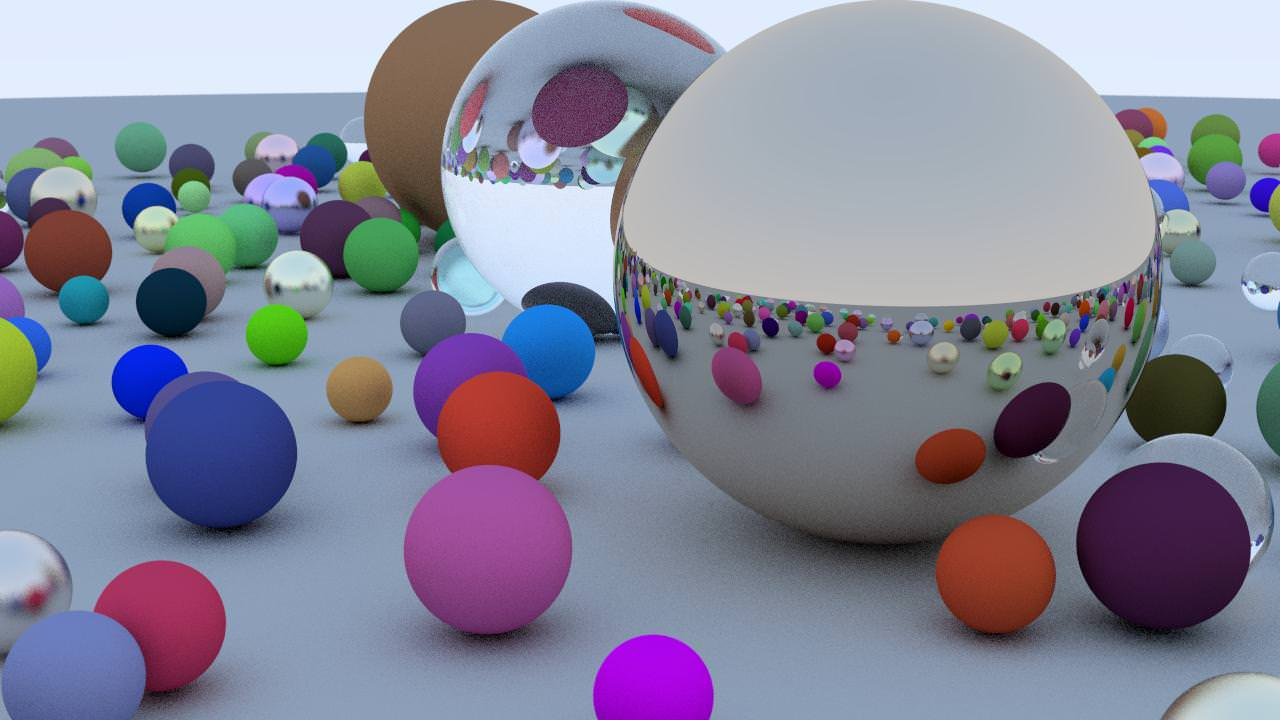
\includegraphics[width=0.8\columnwidth]{figure/session-1/ray-tracer.jpeg}
    \end{figure}
\end{frame}



\begin{frame}{Relationship between architecture and scope} 
    \begin{figure}[t]
        \centering
        \begin{center}               
            \resizebox{0.98\columnwidth}{!}{

\begin{tikzpicture}[]


\node[anchor=north west, inner sep=0pt] (cpu) at (-6.99, 0){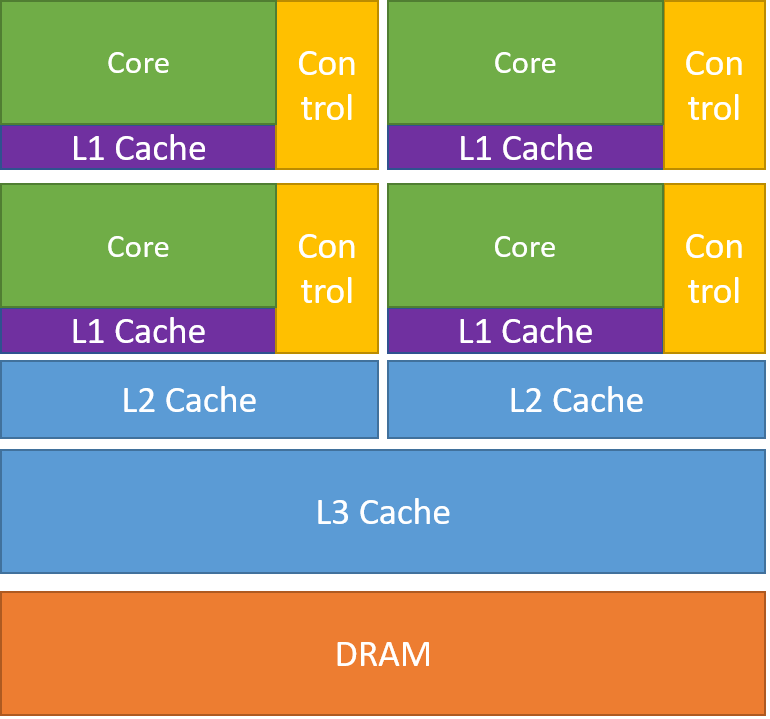
\includegraphics[width=3cm]{figure/session-1/cpu-architecture.png}};
\node[anchor=south] at (cpu.north) {CPU};

\node[anchor=north east, inner sep=0pt] (gpu) at (6.99, 0){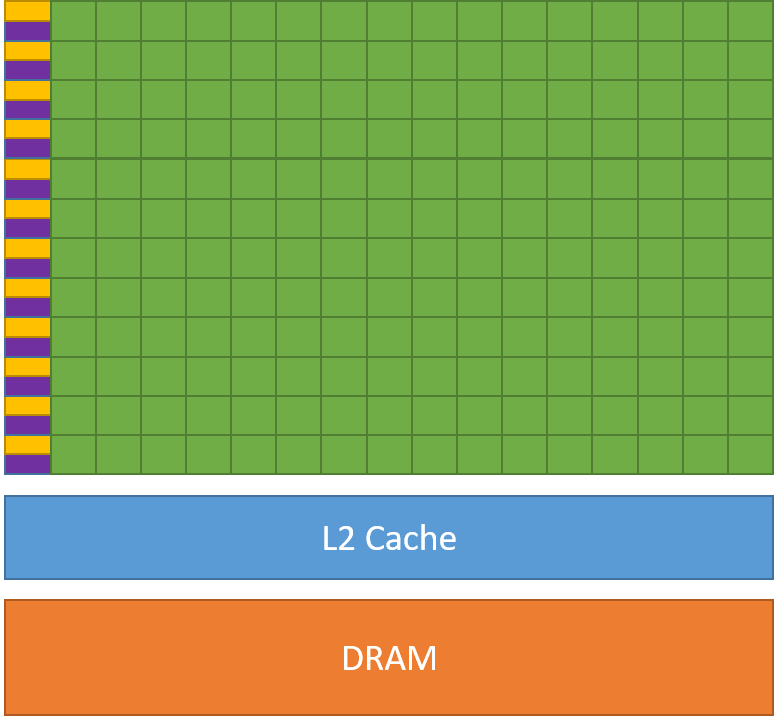
\includegraphics[width=3cm]{figure/session-1/gpu-architecture.png}};
\node[anchor=south] at (gpu.north) {GPU};

\fill[anchor=north, color=black!5!white] (-2.5,0) rectangle ++(5,-2.2);
\fill[anchor=north, color=black!10!white] (-2.5,-2.2) rectangle ++(5,-2.8);
\draw[anchor=north] (-2.5,0) rectangle ++(5,-5);
\node[anchor=south] at (0,0) {code.cpp};


% Top script

\def\topy{-0.35}

\node[anchor=west, align=left, font=\footnotesize] at (-2.4, \topy) {1.};
\node[anchor=west, align=left, font=\footnotesize] at (-2, \topy) {Includes and defines};

\node[anchor=west, align=left, font=\footnotesize] at (-2.4, \topy-0.6) {2.};
\node[anchor=west, align=left, font=\footnotesize] at (-2, \topy-0.6) {CPU functions};
\node[anchor=west, align=left, font=\footnotesize] at (-2, \topy-1.0) {Kernel functions (global)};
\node[anchor=west, align=left, font=\footnotesize, text=OliveGreen] at (-2, \topy-1.4) {GPU functions (device)};



% Bottom script

\def\topy{-2.7}

\node[anchor=west, align=left, font=\footnotesize] at (-2.4, \topy) {3.};
\node[anchor=west, align=left, font=\footnotesize] at (-2, \topy) {Memory alloc. and migration};

\node[anchor=west, align=left, font=\footnotesize] at (-2.4, \topy-0.6) {4.};
\node[anchor=west, align=left, font=\footnotesize] at (-2, \topy-0.6) {Kernel invocation (and timing)};

\node[anchor=west, align=left, font=\footnotesize] at (-2.4, \topy-1.2) {5.};
\node[anchor=west, align=left, font=\footnotesize] at (-2, \topy-1.2) {Memory migration};
\node[anchor=west, align=left, font=\footnotesize] at (-2, \topy-1.6) {(and checking/dumping)};



\draw [decorate, decoration={brace, amplitude=10pt, mirror}] (-2.9,0) -- (-2.9,-5);
% \draw [-{angle 60}] (-3.3, -2.5) -- (-3.8, -2.5);
\node[anchor=center, align=center, font=\footnotesize] at (-5, -3.5) {Compilation/execution \\on the CPU};


\only<2->{
\draw [decorate, decoration={brace, amplitude=10pt}] (1.8,-1.2) -- (1.8,-1.9);
\draw [-{angle 60}] (2.35, -1.55) -- (3.5, -1.55);
\draw [-{angle 60}] (2.1, -2.6) -- (3.5, -2.0);
% \draw [-{angle 60}] (1.6, -4.2) -- (3.5, -2.8);
\draw [-{angle 60}] (1.6, -4.2) -- (3.5, -2.8);
\node[anchor=center, align=center, font=\footnotesize] at (5, -3.5) {Interface to the GPU};
}


\only<3->{
% Bottom script
\draw [-{angle 60}] (-2.4, -3.2) to[out=160, in=-140] (-2.0, -1.45);
\draw [-{angle 60}] (1.45, -1.35) 
to[out=-10, in=90] (1.7, -1.525)
to[out=-90, in=10] (1.3, -1.75);
}


\end{tikzpicture}
}
        \end{center}
    \end{figure}
% textwidth in cm: \printinunitsof{cm}\prntlen{\textwidth}
\end{frame}



\begin{frame}{CUDA, an API for programming Nvidia GPUs}
    \begin{figure}
        \centering
        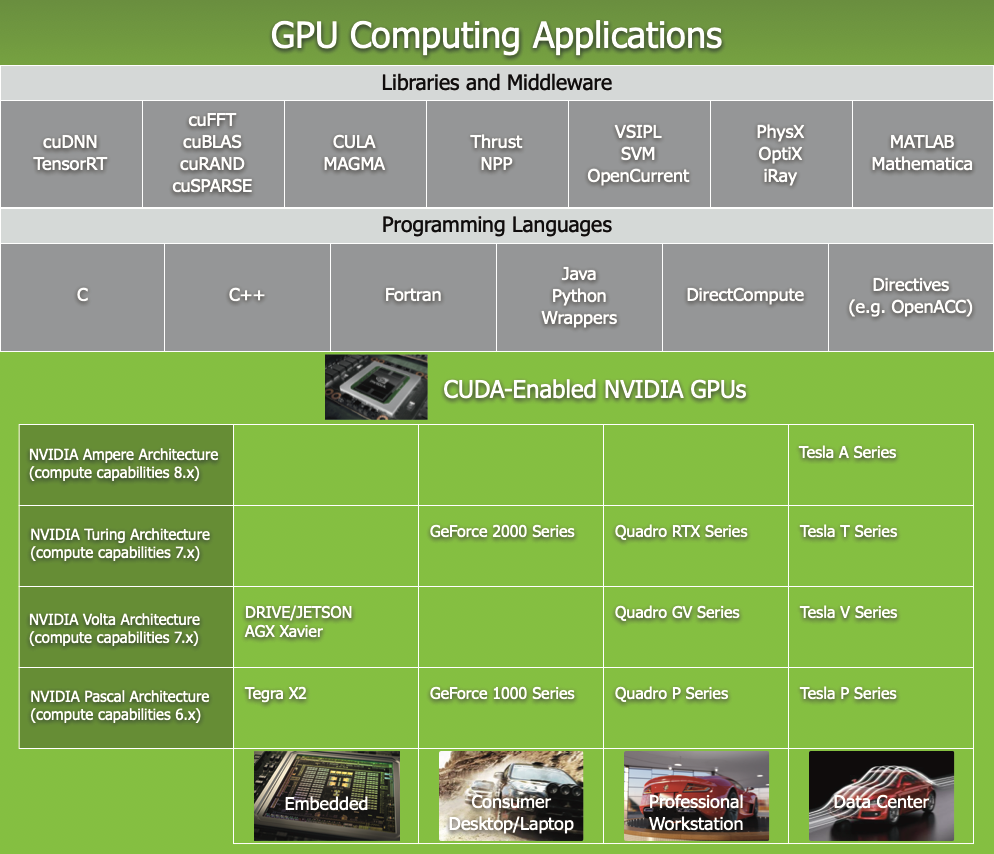
\includegraphics[width=7cm]{figure/session-1/gpu-computing-applications.png}
    \end{figure}	
\end{frame}



\begin{frame}{Environment and workflow} 
    \begin{figure}[t]
        \centering
        \begin{center}               
            \resizebox{0.98\columnwidth}{!}{
\begin{tikzpicture}[]

\node[align=center] (yc) at (-6, 0) {Your code\\(C++)};

\node[align=center] (ide) at (-2, 0) {IDE\\(VSC)};
\draw[black] (ide.south west) rectangle (ide.north east);
\node[align=center] (inst) at (-2, 2) {Instructions\\(tasks.json)};
\node[align=center] (comp) at (-2, -2) {Compiler\\(nvcc))};
\draw[black] (comp.south west) rectangle (comp.north east);

\node[align=center] (cpu) at ( 2, 0) {CPU};
\draw[black] (cpu.south west) rectangle (cpu.north east);
\node[align=center] (gpu) at ( 2, -2) {GPU};
\draw[black] (gpu.south west) rectangle (gpu.north east);

\node[align=center] (term) at ( 6, 2) {Terminal (printf)};
\node[align=center] (dump) at ( 6, 0) {Dump (file)};
\node[align=center] (vir) at ( 6, -2) {Virus (\dots)};


\draw[-{angle 60}] (yc.east) -- (ide.west);

\draw[] (comp.north) -- (ide.south);
\draw[-{angle 60}] (inst.south) -- (ide.north) ;
\draw[-{angle 60}] (ide.east) -- (cpu.west);


\draw[-{angle 60}] (gpu.north) -- (cpu.south);
\draw[-{angle 60}] (cpu.east) -- (term.west);
\draw[-{angle 60}] (cpu.east) -- (dump);
\draw[-{angle 60}] (cpu.east) -- (vir.west);


\end{tikzpicture}}
        \end{center}
    \end{figure}
\end{frame}



\begin{frame}{Organization of the lab and docs} 
    \begin{figure}[t]
        \centering
        \begin{center}               
            \resizebox{0.98\columnwidth}{!}{
\begin{tikzpicture}[]

\node[align=center, anchor=center] (gca) at (0, 0) {GCA lab};



\node[align=center, anchor=center] (docs) at (0, 1.5) {Docs\\(Toledo)};
\node[align=center, anchor=center, font=\footnotesize, text=black!60!white] at (-2, 2.25) {Prog. guide};
\node[align=center, anchor=center, font=\footnotesize, text=black!60!white] at ( 0, 2.5) {Cheat sheet};
\node[align=center, anchor=center, font=\footnotesize, text=black!60!white] at ( 2, 2.25) {tasks.json};



\node[align=center, anchor=center] (sess) at (3, -1) {6 Sessions};
\node[align=center, anchor=center, font=\footnotesize, text=black!60!white] at ( 3, 0 ) {Kernel};
\node[align=center, anchor=center, font=\footnotesize, text=black!60!white] at ( 4.5, 0 ) {Race c.};
\node[align=center, anchor=center, font=\footnotesize, text=black!60!white] at ( 5, -0.75 ) {Warps};
\node[align=center, anchor=center, font=\footnotesize, text=black!60!white] at ( 5, -1.5 ) {Memory};
\node[align=center, anchor=center, font=\footnotesize, text=black!60!white] at ( 4.5, -2.25 ) {Dynamic p.};
\node[align=center, anchor=center, font=\footnotesize, text=black!60!white] at ( 3, -2.25 ) {Async.};



\node[align=center, anchor=center] (proj) at (-3, -1) {Project};
% \node[align=center, anchor=center, font=\footnotesize, text=black!60!white] at ( -3, 0 ) {Graphics};
\node[align=center, anchor=center, font=\footnotesize, text=black!60!white] at ( -4.5, 0 ) {\dots};
\node[align=center, anchor=center, font=\footnotesize, text=black!60!white] at ( -5, -0.75 ) {Encoding};
\node[align=center, anchor=center, font=\footnotesize, text=black!60!white] at ( -5, -1.5 ) {Encryption};
\node[align=center, anchor=center, font=\footnotesize, text=black!60!white] at ( -4.5, -2.25 ) {DSP};
\node[align=center, anchor=center, font=\footnotesize, text=black!60!white] at ( -3, -2.25 ) {Graphics};


\draw[black] (gca.south west) rectangle (gca.north east);

\draw[] (gca.south west) -- (proj.north east);
\draw[] (gca.south east) -- (sess.north west);
\draw[] (gca.north) -- (docs.south);


\end{tikzpicture}
}
        \end{center}
    \end{figure}
\end{frame}



\begin{frame}{Responsibilities and evaluation} 
    \begin{figure}[t]
        \centering
        \begin{center}               
            \resizebox{0.98\columnwidth}{!}{
\begin{tikzpicture}[]

\foreach \i in {0,...,2} {
    \node[anchor=center, align=center, font=\footnotesize] (lr\i) at (-5.5, -1.2*\i) {Single-page report};
    \draw[black] (lr\i.south west) rectangle (lr\i.north east);
    
    \node[anchor=center, align=center, font=\footnotesize] (rr\i) at (-2, -1.2*\i) {Single-page report};
    \draw[black] (rr\i.south west) rectangle (rr\i.north east);
}

\node[anchor=center, align=center, font=\footnotesize] (pr) at (3.5,0) {Project report};
\draw[black] (pr.south west) rectangle (pr.north east);
    
\node[anchor=center, align=center, font=\footnotesize] (pp) at (3.5,-1.2) {Project Presentation};
\draw[black] (pp.south west) rectangle (pp.north east);
    
\node[anchor=center, align=center, font=\footnotesize] (cr) at (3.5,-2.4) {Code release};
\draw[black] (cr.south west) rectangle (cr.north east);


\draw[dashed] (0, 1.5) -- (0, -3);

\node[] at (-3.5, 1) {Lab seesions, 50 \%};
\node[] at ( 3.5, 1) {Project, 50 \%};


\end{tikzpicture}
}
        \end{center}
    \end{figure}
\end{frame}


\begin{frame}{Recap} 

    \vspace{-0.5cm}

    \begin{columns}[t] % align columns at the top
    \column{0.5\textwidth} % first column
    \begin{figure}
    \centering
    \resizebox{0.95\columnwidth}{!}{

\begin{tikzpicture}[]


\node[anchor=north west, inner sep=0pt] (cpu) at (-6.99, 0){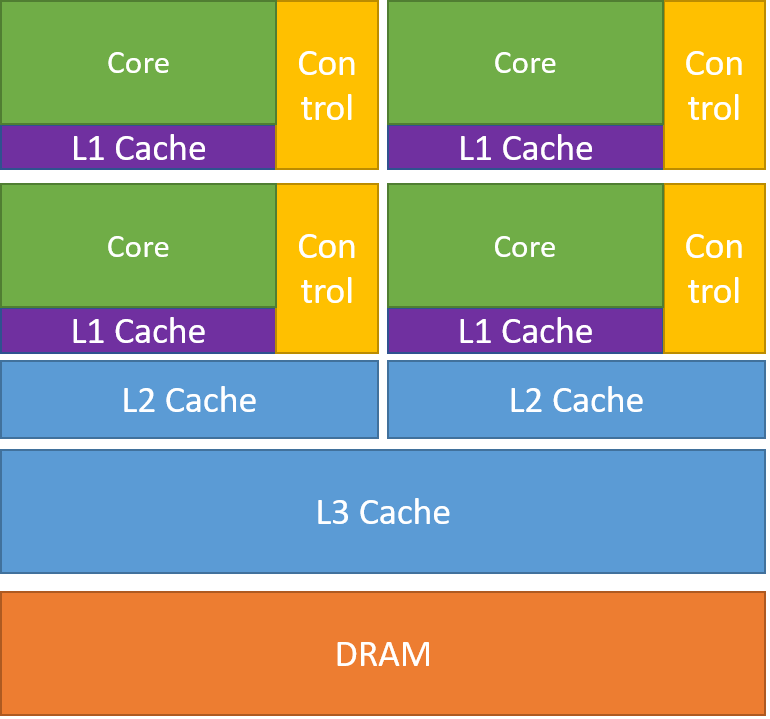
\includegraphics[width=3cm]{figure/session-1/cpu-architecture.png}};
\node[anchor=south] at (cpu.north) {CPU};

\node[anchor=north east, inner sep=0pt] (gpu) at (6.99, 0){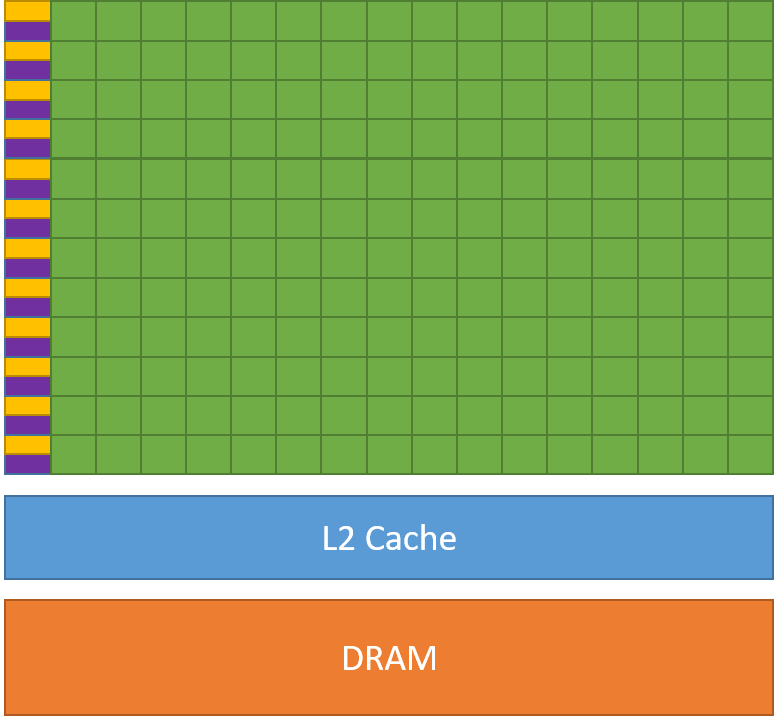
\includegraphics[width=3cm]{figure/session-1/gpu-architecture.png}};
\node[anchor=south] at (gpu.north) {GPU};

\fill[anchor=north, color=black!5!white] (-2.5,0) rectangle ++(5,-2.2);
\fill[anchor=north, color=black!10!white] (-2.5,-2.2) rectangle ++(5,-2.8);
\draw[anchor=north] (-2.5,0) rectangle ++(5,-5);
\node[anchor=south] at (0,0) {code.cpp};


% Top script

\def\topy{-0.35}

\node[anchor=west, align=left, font=\footnotesize] at (-2.4, \topy) {1.};
\node[anchor=west, align=left, font=\footnotesize] at (-2, \topy) {Includes and defines};

\node[anchor=west, align=left, font=\footnotesize] at (-2.4, \topy-0.6) {2.};
\node[anchor=west, align=left, font=\footnotesize] at (-2, \topy-0.6) {CPU functions};
\node[anchor=west, align=left, font=\footnotesize] at (-2, \topy-1.0) {Kernel functions (global)};
\node[anchor=west, align=left, font=\footnotesize, text=OliveGreen] at (-2, \topy-1.4) {GPU functions (device)};



% Bottom script

\def\topy{-2.7}

\node[anchor=west, align=left, font=\footnotesize] at (-2.4, \topy) {3.};
\node[anchor=west, align=left, font=\footnotesize] at (-2, \topy) {Memory alloc. and migration};

\node[anchor=west, align=left, font=\footnotesize] at (-2.4, \topy-0.6) {4.};
\node[anchor=west, align=left, font=\footnotesize] at (-2, \topy-0.6) {Kernel invocation (and timing)};

\node[anchor=west, align=left, font=\footnotesize] at (-2.4, \topy-1.2) {5.};
\node[anchor=west, align=left, font=\footnotesize] at (-2, \topy-1.2) {Memory migration};
\node[anchor=west, align=left, font=\footnotesize] at (-2, \topy-1.6) {(and checking/dumping)};



\draw [decorate, decoration={brace, amplitude=10pt, mirror}] (-2.9,0) -- (-2.9,-5);
% \draw [-{angle 60}] (-3.3, -2.5) -- (-3.8, -2.5);
\node[anchor=center, align=center, font=\footnotesize] at (-5, -3.5) {Compilation/execution \\on the CPU};


\draw [decorate, decoration={brace, amplitude=10pt}] (1.8,-1.2) -- (1.8,-1.9);
\draw [-{angle 60}] (2.35, -1.55) -- (3.5, -1.55);
\draw [-{angle 60}] (2.1, -2.6) -- (3.5, -2.0);
% \draw [-{angle 60}] (1.6, -4.2) -- (3.5, -2.8);
\draw [-{angle 60}] (1.6, -4.2) -- (3.5, -2.8);
\node[anchor=center, align=center, font=\footnotesize] at (5, -3.5) {Interface to the GPU};



% Bottom script
\draw [-{angle 60}] (-2.4, -3.2) to[out=160, in=-140] (-2.0, -1.45);
\draw [-{angle 60}] (1.45, -1.35) 
to[out=-10, in=90] (1.7, -1.525)
to[out=-90, in=10] (1.3, -1.75);


\end{tikzpicture}
}
    \end{figure}
    
    \column{0.5\textwidth} % second column
    \begin{figure}
    \centering
    \resizebox{0.95\columnwidth}{!}{
\begin{tikzpicture}[]

\node[align=center] (yc) at (-6, 0) {Your code\\(C++)};

\node[align=center] (ide) at (-2, 0) {IDE\\(VSC)};
\draw[black] (ide.south west) rectangle (ide.north east);
\node[align=center] (inst) at (-2, 2) {Instructions\\(tasks.json)};
\node[align=center] (comp) at (-2, -2) {Compiler\\(nvcc))};
\draw[black] (comp.south west) rectangle (comp.north east);

\node[align=center] (cpu) at ( 2, 0) {CPU};
\draw[black] (cpu.south west) rectangle (cpu.north east);
\node[align=center] (gpu) at ( 2, -2) {GPU};
\draw[black] (gpu.south west) rectangle (gpu.north east);

\node[align=center] (term) at ( 6, 2) {Terminal (printf)};
\node[align=center] (dump) at ( 6, 0) {Dump (file)};
\node[align=center] (vir) at ( 6, -2) {Virus (\dots)};


\draw[-{angle 60}] (yc.east) -- (ide.west);

\draw[] (comp.north) -- (ide.south);
\draw[-{angle 60}] (inst.south) -- (ide.north) ;
\draw[-{angle 60}] (ide.east) -- (cpu.west);


\draw[-{angle 60}] (gpu.north) -- (cpu.south);
\draw[-{angle 60}] (cpu.east) -- (term.west);
\draw[-{angle 60}] (cpu.east) -- (dump);
\draw[-{angle 60}] (cpu.east) -- (vir.west);


\end{tikzpicture}}
    \end{figure}
    \end{columns}
    
    \begin{columns}[t] % align columns at the top
    \column{0.5\textwidth} % first column
    \begin{figure}
    \centering
    \resizebox{0.95\columnwidth}{!}{
\begin{tikzpicture}[]

\node[align=center, anchor=center] (gca) at (0, 0) {GCA lab};



\node[align=center, anchor=center] (docs) at (0, 1.5) {Docs\\(Toledo)};
\node[align=center, anchor=center, font=\footnotesize, text=black!60!white] at (-2, 2.25) {Prog. guide};
\node[align=center, anchor=center, font=\footnotesize, text=black!60!white] at ( 0, 2.5) {Cheat sheet};
\node[align=center, anchor=center, font=\footnotesize, text=black!60!white] at ( 2, 2.25) {tasks.json};



\node[align=center, anchor=center] (sess) at (3, -1) {6 Sessions};
\node[align=center, anchor=center, font=\footnotesize, text=black!60!white] at ( 3, 0 ) {Kernel};
\node[align=center, anchor=center, font=\footnotesize, text=black!60!white] at ( 4.5, 0 ) {Race c.};
\node[align=center, anchor=center, font=\footnotesize, text=black!60!white] at ( 5, -0.75 ) {Warps};
\node[align=center, anchor=center, font=\footnotesize, text=black!60!white] at ( 5, -1.5 ) {Memory};
\node[align=center, anchor=center, font=\footnotesize, text=black!60!white] at ( 4.5, -2.25 ) {Dynamic p.};
\node[align=center, anchor=center, font=\footnotesize, text=black!60!white] at ( 3, -2.25 ) {Async.};



\node[align=center, anchor=center] (proj) at (-3, -1) {Project};
% \node[align=center, anchor=center, font=\footnotesize, text=black!60!white] at ( -3, 0 ) {Graphics};
\node[align=center, anchor=center, font=\footnotesize, text=black!60!white] at ( -4.5, 0 ) {\dots};
\node[align=center, anchor=center, font=\footnotesize, text=black!60!white] at ( -5, -0.75 ) {Encoding};
\node[align=center, anchor=center, font=\footnotesize, text=black!60!white] at ( -5, -1.5 ) {Encryption};
\node[align=center, anchor=center, font=\footnotesize, text=black!60!white] at ( -4.5, -2.25 ) {DSP};
\node[align=center, anchor=center, font=\footnotesize, text=black!60!white] at ( -3, -2.25 ) {Graphics};


\draw[black] (gca.south west) rectangle (gca.north east);

\draw[] (gca.south west) -- (proj.north east);
\draw[] (gca.south east) -- (sess.north west);
\draw[] (gca.north) -- (docs.south);


\end{tikzpicture}
}
    \end{figure}
    
    \column{0.5\textwidth} % second column
    \begin{figure}
    \centering
    \resizebox{0.95\columnwidth}{!}{
\begin{tikzpicture}[]

\foreach \i in {0,...,2} {
    \node[anchor=center, align=center, font=\footnotesize] (lr\i) at (-5.5, -1.2*\i) {Single-page report};
    \draw[black] (lr\i.south west) rectangle (lr\i.north east);
    
    \node[anchor=center, align=center, font=\footnotesize] (rr\i) at (-2, -1.2*\i) {Single-page report};
    \draw[black] (rr\i.south west) rectangle (rr\i.north east);
}

\node[anchor=center, align=center, font=\footnotesize] (pr) at (3.5,0) {Project report};
\draw[black] (pr.south west) rectangle (pr.north east);
    
\node[anchor=center, align=center, font=\footnotesize] (pp) at (3.5,-1.2) {Project Presentation};
\draw[black] (pp.south west) rectangle (pp.north east);
    
\node[anchor=center, align=center, font=\footnotesize] (cr) at (3.5,-2.4) {Code release};
\draw[black] (cr.south west) rectangle (cr.north east);


\draw[dashed] (0, 1.5) -- (0, -3);

\node[] at (-3.5, 1) {Lab seesions, 50 \%};
\node[] at ( 3.5, 1) {Project, 50 \%};


\end{tikzpicture}
}
    \end{figure}
    \end{columns}

\end{frame}



\section{A grid of threads}

\begin{frame}{Threads are organized into a grid} 

    \begin{figure}[t]
        \centering
        \begin{center}               
            \resizebox{0.98\columnwidth}{!}{

\begin{tikzpicture}[]


%%% DEFINITIONS %%%%%%%%%%%%%%%%%%%%%%%%%%%%%%%%%%%%%%%%%%%%%%%%%%%%%%%%%%%%%


% https://associatie.kuleuven.be/huisstijl/kleuren
\definecolor{blue1}{RGB}{82,189,236}
\definecolor{blue2}{RGB}{0,64,122}
\definecolor{blue3}{RGB}{31,171,231}
\definecolor{blue4}{RGB}{29,141,176}
\definecolor{blue5}{RGB}{17,110,138}
\definecolor{orange1}{RGB}{221,138,46}


\def\ThPoolCenterOneX{-2}
\def\ThPoolCenterOneY{0}

\def\ThPoolCenterTwoX{-5}
\def\ThPoolCenterTwoY{0}


%%% DRAWING %%%%%%%%%%%%%%%%%%%%%%%%%%%%%%%%%%%%%%%%%%%%%%%%%%%%%%%%%%%%%%%%%



\filldraw [blue2, opacity=0.1] (\ThPoolCenterTwoX+1.8,\ThPoolCenterOneY) circle (2.8);

\foreach \x in {1,...,6} {
    \node[inner sep=0pt] at (\ThPoolCenterTwoX+\x/2, 1.5){
\includegraphics[width=0.25cm]{figure/session-1/thread-small.png}};
}
\foreach \x in {-1,...,8} {
    \node[inner sep=0pt] at (\ThPoolCenterTwoX+\x/2, 0){
\includegraphics[width=0.25cm]{figure/session-1/thread-small.png}};
}
\foreach \x in {1,...,6} {
    \node[inner sep=0pt] at (\ThPoolCenterTwoX+\x/2, -1.5){
\includegraphics[width=0.25cm]{figure/session-1/thread-small.png}};
}

% Full grid, threads
\foreach \x in {0,...,3} {
    \draw[black, dashed] (4.5+\x,0.5) rectangle ++(1,-1);
    \node[anchor=center] at (4.5+\x+0.5,0){
\includegraphics[width=0.25cm]{figure/session-1/thread-small.png}};
}

% Blocks
\foreach \x in {0,...,1} {
    \draw[black, very thick] (4.5+2*\x,0.5) rectangle ++(2,-1);
}


\node[] at (-3.25, 3.25) {Pool};
\node[] at ( 6.50, 1.25) {Grid};

\draw[-{angle 60}] (0,0) -- (4,0);



\node[] at ( 3.50, 2.75) {{\color{red}Two blocks}, each with {\color{blue}two threads}};

\node[] at ( 3.50, 2.25) {foo\lstinline[language=C++]{<<<}{\color{red}2}, {\color{blue}2}\lstinline[language=C++]{>>>}(arg1, arg2, \dots)};


\end{tikzpicture}
}
        \end{center}
    \end{figure}
    
\end{frame}



\begin{frame}{Calling a kernel function -- example} 

    \vspace{0.5 em}
    Goal:
    \begin{small}
    \begin{itemize}
        \item Process each input element using exactly one thread {\footnotesize (not always the case)}
    \end{itemize}
    \end{small}
    
    \vspace{0.5 em}
    
    Open questions (OQs):
    \begin{small}
    \begin{enumerate}
        \item How would you define the block- and grid size? {\footnotesize (\# threads in block and \# blocks in grid)}
        \item How does a thread know which element it should process?
    \end{enumerate}
    \end{small}
    
    \vspace{0.5 em}
    
    \begin{figure}[t]
        \centering
        \begin{center}               
            \resizebox{0.8\columnwidth}{!}{

\begin{tikzpicture}[]


%%% DEFINITIONS %%%%%%%%%%%%%%%%%%%%%%%%%%%%%%%%%%%%%%%%%%%%%%%%%%%%%%%%%%%%%


% https://associatie.kuleuven.be/huisstijl/kleuren
\definecolor{blue1}{RGB}{82,189,236}
\definecolor{blue2}{RGB}{0,64,122}
\definecolor{blue3}{RGB}{31,171,231}
\definecolor{blue4}{RGB}{29,141,176}
\definecolor{blue5}{RGB}{17,110,138}
\definecolor{orange1}{RGB}{221,138,46}


\def\SignalY{2}
\def\GridY{0}
\def\MultiplierX{1.2}

\def\SquareSize{1}

\def\ThPoolCenterTwoX{2}
\def\ThPoolCenterTwoY{0}

\def\NumOfSamples{12}

\def\BlockDimX{4}


%%% DRAWING %%%%%%%%%%%%%%%%%%%%%%%%%%%%%%%%%%%%%%%%%%%%%%%%%%%%%%%%%%%%%%%%%



\foreach \x in {0,...,11} {
    \draw[black] (\x * \MultiplierX, \SignalY) rectangle ++ (\SquareSize, \SquareSize);
    \node at (\x * \MultiplierX + \SquareSize/2, \SignalY + \SquareSize/2) {in$_{\x}$};
    \draw[<-] (\x * \MultiplierX + \SquareSize/2, \SignalY - 0.1) -- (\x * \MultiplierX + \SquareSize/2, \GridY + \SquareSize + 0.3);
    \node[inner sep=0pt] at (\x * \MultiplierX + \SquareSize/2, \SignalY - 1.5){
\includegraphics[width=1em]{figure/session-1/thread-small.png}};
}


\end{tikzpicture}}
        \end{center}
    \end{figure}

\end{frame}



\begin{frame}[fragile]{OQ$_\text{1}$: You decide how to divide the grid} 

\begin{lstlisting}[language=C++]
foo<<<1, 12>>>(input_data, output_data)
foo<<<3, 4>>>(input_data, output_data)
\end{lstlisting}

\begin{figure}[t]
    \centering
    \begin{center}               
        \resizebox{0.8\columnwidth}{!}{

\begin{tikzpicture}[]


%%% DEFINITIONS %%%%%%%%%%%%%%%%%%%%%%%%%%%%%%%%%%%%%%%%%%%%%%%%%%%%%%%%%%%%%


% https://associatie.kuleuven.be/huisstijl/kleuren
\definecolor{blue1}{RGB}{82,189,236}
\definecolor{blue2}{RGB}{0,64,122}
\definecolor{blue3}{RGB}{31,171,231}
\definecolor{blue4}{RGB}{29,141,176}
\definecolor{blue5}{RGB}{17,110,138}
\definecolor{orange1}{RGB}{221,138,46}


\def\SignalY{2}
\def\GridOneY{-3.5}
\def\GridTwoY{0}
\def\MultiplierX{1.2}

\def\SquareSize{1}

\def\ThPoolCenterTwoX{2}
\def\ThPoolCenterTwoY{0}

\def\NumOfSamples{12}

\def\BlockDimX{4}


%%% DRAWING %%%%%%%%%%%%%%%%%%%%%%%%%%%%%%%%%%%%%%%%%%%%%%%%%%%%%%%%%%%%%%%%%



\foreach \b in {0,...,2} {
    \foreach \t in {0,...,3} {
        \pgfmathsetmacro{\res}{int(\t+\BlockDimX*\b)}
        \draw[black] ({(\t + \b * \BlockDimX) * \MultiplierX}, \GridOneY) rectangle ++ (\SquareSize, \SquareSize);
        \node at ({(\t + \SquareSize * \b * \BlockDimX) * \MultiplierX + \SquareSize/2}, \GridOneY + \SquareSize/2) {t$_{\t}$};
    }
    \draw[black] (-0.1 + \b * \MultiplierX * \BlockDimX, \GridOneY - 0.1 - 0.6) rectangle ++ (\SquareSize * \MultiplierX * \BlockDimX, \SquareSize + 0.2 + 0.6);
    \node at ({(\b + 0.5) * \MultiplierX * \BlockDimX}, \GridOneY - 0.45) {block$_\b$};
}


\draw[black, very thick] (-0.2, \GridOneY - 0.2 - 0.6 - 0.6) rectangle ++ (\SquareSize * \MultiplierX * \NumOfSamples + 0.2, \SquareSize + 0.4 + 0.6 + 0.6);
\node at (0.3, \GridOneY-1.1) {grid};

\node[rotate=90] at (-0.75, \GridOneY) {[3, 4]};
\node[rotate=90] at (\SquareSize * \MultiplierX * \NumOfSamples + 0.5, \GridOneY) {[3, 4]};




\foreach \x in {0,...,11} {
    \draw[black] (\x * \MultiplierX, \GridTwoY) rectangle ++ (\SquareSize, \SquareSize);
    \node at (\x * \MultiplierX + \SquareSize/2, \GridTwoY + \SquareSize/2) {t$_{\x}$};
}

\draw[black] (-0.1, \GridTwoY - 0.7) rectangle ++ (\SquareSize * \MultiplierX * \NumOfSamples, \SquareSize + 0.8);
\node at ({1.5 * \MultiplierX * \BlockDimX}, \GridTwoY - 0.45) {block$_0$};

\draw[black, very thick] (-0.2, \GridTwoY - 1.4) rectangle ++ (\SquareSize * \MultiplierX * \NumOfSamples + 0.2, \SquareSize + 1.6);
\node at (0.3, \GridTwoY-1.1) {grid};

\node[rotate=90] at (-0.75, \GridTwoY) {[1, 12]};
\node[rotate=90] at (\SquareSize * \MultiplierX * \NumOfSamples + 0.5, \GridTwoY) {[1, 12]};



\end{tikzpicture}}
    \end{center}
\end{figure}

\end{frame}



\begin{frame}[fragile]{OQ$_\text{2}$: Importance of correct indexing} 

\begin{lstlisting}[language=C++]
foo<<<1, 12>>>(input_data, output_data)
\end{lstlisting}

\vspace{-0 em}

\begin{figure}[t]
    \centering
    \begin{center}               
        \resizebox{0.8\columnwidth}{!}{

\begin{tikzpicture}[]


%%% DEFINITIONS %%%%%%%%%%%%%%%%%%%%%%%%%%%%%%%%%%%%%%%%%%%%%%%%%%%%%%%%%%%%%


% https://associatie.kuleuven.be/huisstijl/kleuren
\definecolor{blue1}{RGB}{82,189,236}
\definecolor{blue2}{RGB}{0,64,122}
\definecolor{blue3}{RGB}{31,171,231}
\definecolor{blue4}{RGB}{29,141,176}
\definecolor{blue5}{RGB}{17,110,138}
\definecolor{orange1}{RGB}{221,138,46}


\def\SignalY{2}
% \def\GridOneY{0}
\def\GridOneY{-2}
\def\GridTwoY{-1.5}
\def\MultiplierX{1.2}

\def\SquareSize{1}

\def\ThPoolCenterTwoX{2}
\def\ThPoolCenterTwoY{0}

\def\NumOfSamples{12}

\def\BlockDimX{4}


%%% DRAWING %%%%%%%%%%%%%%%%%%%%%%%%%%%%%%%%%%%%%%%%%%%%%%%%%%%%%%%%%%%%%%%%%



\foreach \x in {0,...,11} {
    \draw[black] (\x * \MultiplierX, \SignalY) rectangle ++ (\SquareSize, \SquareSize);
    \node at (\x * \MultiplierX + \SquareSize/2, \SignalY + \SquareSize/2) {in$_{\x}$};
    \draw[<-] (\x * \MultiplierX + \SquareSize/2, \SignalY - 0.1) -- (\x * \MultiplierX + \SquareSize/2, \GridTwoY + \SquareSize + 0.3);
}


\foreach \x in {0,...,11} {
    \draw[black] (\x * \MultiplierX, \GridTwoY) rectangle ++ (\SquareSize, \SquareSize);
    \node at (\x * \MultiplierX + \SquareSize/2, \GridTwoY + \SquareSize/2) {t$_{\x}$};
}

\draw[black] (-0.1, \GridTwoY - 0.7) rectangle ++ (\SquareSize * \MultiplierX * \NumOfSamples, \SquareSize + 0.8);
\node at ({1.5 * \MultiplierX * \BlockDimX}, \GridTwoY - 0.45) {block$_0$};

\draw[black, very thick] (-0.2, \GridTwoY - 1.4) rectangle ++ (\SquareSize * \MultiplierX * \NumOfSamples + 0.2, \SquareSize + 1.6);
\node at (0.3, \GridTwoY-1.1) {grid};

\node[rotate=90] at (-0.75, \GridTwoY) {[1, 12]};
\node[rotate=90] at (\SquareSize * \MultiplierX * \NumOfSamples + 0.5, \GridTwoY) {[1, 12]};


\end{tikzpicture}}
    \end{center}
\end{figure}

Good: each thread handles exactly one element.

\end{frame}



\begin{frame}[fragile]{OQ$_\text{2}$: Importance of correct indexing} 

\begin{lstlisting}[language=C++]
foo<<<3, 4>>>(input_data, output_data)
\end{lstlisting}

\vspace{-1 em}

\begin{figure}[t]
    \centering
    \begin{center}               
        \resizebox{0.8\columnwidth}{!}{

\begin{tikzpicture}[]


%%% DEFINITIONS %%%%%%%%%%%%%%%%%%%%%%%%%%%%%%%%%%%%%%%%%%%%%%%%%%%%%%%%%%%%%


% https://associatie.kuleuven.be/huisstijl/kleuren
\definecolor{blue1}{RGB}{82,189,236}
\definecolor{blue2}{RGB}{0,64,122}
\definecolor{blue3}{RGB}{31,171,231}
\definecolor{blue4}{RGB}{29,141,176}
\definecolor{blue5}{RGB}{17,110,138}
\definecolor{orange1}{RGB}{221,138,46}


\def\SignalY{2}
% \def\GridOneY{0}
\def\GridOneY{-1.5}
\def\GridTwoY{-3}
\def\MultiplierX{1.2}

\def\SquareSize{1}

\def\ThPoolCenterTwoX{2}
\def\ThPoolCenterTwoY{0}

\def\NumOfSamples{12}

\def\BlockDimX{4}


%%% DRAWING %%%%%%%%%%%%%%%%%%%%%%%%%%%%%%%%%%%%%%%%%%%%%%%%%%%%%%%%%%%%%%%%%



\foreach \x in {0,...,11} {
    \draw[black] (\x * \MultiplierX, \SignalY) rectangle ++ (\SquareSize, \SquareSize);
    \node at (\x * \MultiplierX + \SquareSize/2, \SignalY + \SquareSize/2) {in$_{\x}$};
}


\foreach \x in {0,...,11} {
    \draw[black] (\x * \MultiplierX, \GridOneY) rectangle ++ (\SquareSize, \SquareSize);
}

\foreach \x in {0,...,3} {
    \node at (\x * \MultiplierX + \SquareSize/2, \GridOneY + \SquareSize/2) {t$_{\x}$};
    \draw[<-] (\x * \MultiplierX + \SquareSize/2, \SignalY - 0.1) -- (\x * \MultiplierX + \SquareSize/2, \GridOneY + \SquareSize + 0.3);
}

\foreach \x in {0,...,3} {
    \node at (\x * \MultiplierX + \SquareSize/2 + \SquareSize * \MultiplierX * 4, \GridOneY + \SquareSize/2) {t$_{\x}$};
    \draw[red, <-] (\x * \MultiplierX + \SquareSize/2, \SignalY - 0.1) to [out=-90, in=90] (\x * \MultiplierX + \SquareSize/2 + \SquareSize * \MultiplierX * 4, \GridOneY + \SquareSize + 0.3);
    % \draw[red, <-] (\x * \MultiplierX + \SquareSize/2, \SignalY - 0.1) -- (\x * \MultiplierX + \SquareSize/2 + \SquareSize * \MultiplierX * 4, \GridOneY + \SquareSize + 0.3);
}

\foreach \x in {0,...,3} {
    \node at (\x * \MultiplierX + \SquareSize/2 + \SquareSize * \MultiplierX * 8, \GridOneY + \SquareSize/2) {t$_{\x}$};
    \draw[red, <-] (\x * \MultiplierX + \SquareSize/2, \SignalY - 0.1) to [out=-90, in=90] (\x * \MultiplierX + \SquareSize/2 + \SquareSize * \MultiplierX * 8, \GridOneY + \SquareSize + 0.3);
    % \draw[red, <-] (\x * \MultiplierX + \SquareSize/2, \SignalY - 0.1) -- (\x * \MultiplierX + \SquareSize/2 + \SquareSize * \MultiplierX * 8, \GridOneY + \SquareSize + 0.3);
}


\foreach \x in {0,...,2} {
    \draw[black] (-0.1 + \x * \MultiplierX * \BlockDimX, \GridOneY - 0.1 - 0.6) rectangle ++ (\SquareSize * \MultiplierX * \BlockDimX, \SquareSize + 0.2 + 0.6);
    \node at ({(\x + 0.5) * \MultiplierX * \BlockDimX}, \GridOneY - 0.45) {block$_\x$};
}


\draw[black, very thick] (-0.2, \GridOneY - 0.2 - 0.6 - 0.6) rectangle ++ (\SquareSize * \MultiplierX * \NumOfSamples + 0.2, \SquareSize + 0.4 + 0.6 + 0.6);
\node at (0.3, \GridOneY-1.1) {grid};

\node[rotate=90] at (-0.75, \GridOneY) {[3, 4]};
\node[rotate=90] at (\SquareSize * \MultiplierX * \NumOfSamples + 0.5, \GridOneY) {[3, 4]};


\end{tikzpicture}}
    \end{center}
\end{figure}

Problem: overwriting existing- and skipping elements.

\end{frame}



\begin{frame}[fragile]{OQ$_\text{2}$: Correct indexing} 

\begin{small}
\begin{itemize}
    \item Thread's position within block not enough -- relative position only
    \item Include offset, equal to block size -- calculate absolute position within grid
\end{itemize}
\end{small}

\begin{figure}[t]
    \centering
    \begin{center}               
        \resizebox{0.8\columnwidth}{!}{

\begin{tikzpicture}[]


%%% DEFINITIONS %%%%%%%%%%%%%%%%%%%%%%%%%%%%%%%%%%%%%%%%%%%%%%%%%%%%%%%%%%%%%


% https://associatie.kuleuven.be/huisstijl/kleuren
\definecolor{blue1}{RGB}{82,189,236}
\definecolor{blue2}{RGB}{0,64,122}
\definecolor{blue3}{RGB}{31,171,231}
\definecolor{blue4}{RGB}{29,141,176}
\definecolor{blue5}{RGB}{17,110,138}
\definecolor{orange1}{RGB}{221,138,46}


\def\SignalY{2}
% \def\GridOneY{0}
\def\GridOneY{-1.5}
\def\GridTwoY{-3}
\def\MultiplierX{1.2}

\def\SquareSize{1}

\def\ThPoolCenterTwoX{2}
\def\ThPoolCenterTwoY{0}

\def\NumOfSamples{12}

\def\BlockDimX{4}


%%% DRAWING %%%%%%%%%%%%%%%%%%%%%%%%%%%%%%%%%%%%%%%%%%%%%%%%%%%%%%%%%%%%%%%%%



\foreach \x in {0,...,11} {
    \draw[black] (\x * \MultiplierX, \SignalY) rectangle ++ (\SquareSize, \SquareSize);
    \node at (\x * \MultiplierX + \SquareSize/2, \SignalY + \SquareSize/2) {in$_{\x}$};
    \draw[<-] (\x * \MultiplierX + \SquareSize/2, \SignalY - 0.1) -- (\x * \MultiplierX + \SquareSize/2, \GridOneY + \SquareSize + 0.3);
}


\foreach \b in {0,...,2} {
    \foreach \t in {0,...,3} {
        \pgfmathsetmacro{\res}{int(\t+\BlockDimX*\b)}
        \draw[black] ({(\t + \b * \BlockDimX) * \MultiplierX}, \GridOneY) rectangle ++ (\SquareSize, \SquareSize);
        \node at ({(\t + \SquareSize * \b * \BlockDimX) * \MultiplierX + \SquareSize/2}, \GridOneY + \SquareSize/2) {t$_{\t}$};
        \node [blue2] at ({(\t + \SquareSize * \b * \BlockDimX) * \MultiplierX + \SquareSize/2 + 0.25}, \SignalY - 1.1) {\res};
    }
    \draw[black] (-0.1 + \b * \MultiplierX * \BlockDimX, \GridOneY - 0.1 - 0.6) rectangle ++ (\SquareSize * \MultiplierX * \BlockDimX, \SquareSize + 0.2 + 0.6);
    \node at ({(\b + 0.5) * \MultiplierX * \BlockDimX}, \GridOneY - 0.45) {block$_\b$};
}


\draw[black, very thick] (-0.2, \GridOneY - 0.2 - 0.6 - 0.6) rectangle ++ (\SquareSize * \MultiplierX * \NumOfSamples + 0.2, \SquareSize + 0.4 + 0.6 + 0.6);
\node at (0.3, \GridOneY-1.1) {grid};

\node[rotate=90] at (-0.75, \GridOneY) {[3, 4]};
\node[rotate=90] at (\SquareSize * \MultiplierX * \NumOfSamples + 0.5, \GridOneY) {[3, 4]};


\end{tikzpicture}}
    \end{center}
\end{figure}

\end{frame}



\begin{frame}{Useful built-in functions} 

\vspace{0.75 em}

\begin{itemize}
    \setlength\itemsep{0.5 em}
    \item Thread's index within the block \inline{threadIdx.x}
    \item Block's index within the grid \inline{blockIdx.x}
    \item Block's size (\# threads in block) \inline{blockDim.x}
    \item Grid's size  (\# blocks in grid)\inline{gridDim.x}
\end{itemize}

\vspace{1cm}

What is the largest possible block size (max. threads per block)?

See p. 12 of the reference guide.

\end{frame}




\section{Exercise}


\begin{frame}{First session's exercise} 

    \vspace{0.25cm}

    \begin{columns}[t] % align columns at the top
    \column{0.6\textwidth} % first column
    \textbf{Problem}
    \begin{itemize}\setlength\itemsep{0.5em}
        \item Flip array
        \item Use multiple blocks with multiple threads
    \end{itemize}
    
    \column{0.4\textwidth} % second column

    \begin{figure}[t]
        \centering
        \begin{center}               
            \resizebox{0.98\columnwidth}{!}{

\begin{tikzpicture}[]




% Full grid, threads
\foreach \x in {0,...,8} {

    \draw[black] (0.5*\x,1.0) rectangle ++(0.5,-0.5);
    \node[] at (0.5*\x+0.25,1.0-0.25) {\x};
    
    \draw[black] (4-0.5*\x,0.0) rectangle ++(0.5,-0.5);
    \node[] at (4-0.5*\x+0.25,-0.25) {\x};

    \node[anchor=west, align=left] at (-1.25,  0.75) {In:};
    \node[anchor=west, align=left] at (-1.25, -0.25) {Out:};
    
}



\end{tikzpicture}
}
        \end{center}
    \end{figure}
    
    \end{columns}


    \vspace{0.5cm}
    
    \textbf{Goal}
    \begin{itemize}\setlength\itemsep{0.5em}
        \item Write and execute parallel code on the GPU
        \item Migrate memory and verify the results (flipping)
    \end{itemize}

    \vspace{0.5cm}
    
    Reports are due by your next lab session.
    

\end{frame}




\appendix
\begin{frame}[noframenumbering,label=extraframe]{Extra slide}


\begin{footnotesize}

Images and figures borrowed from:

\begin{itemize}
    \item \url{https://github.com/mellinoe/veldrid-raytracer}
    \item \url{https://docs.nvidia.com/cuda/cuda-c-programming-guide/index.html}
\end{itemize}

\end{footnotesize}


\end{frame}


\end{document}
